% !TeX spellcheck = en_US
% !TeX encoding = UTF-8
\documentclass[a4paper]{article}
\usepackage{graphics, graphicx}
\usepackage{fancyvrb, enumerate}
\usepackage{amsmath, amssymb, amscd, amsfonts}
\usepackage{geometry}
\usepackage{multirow}
\usepackage{url}
\usepackage{listings, listing}
\usepackage{color}
\usepackage{mathptmx}
\usepackage[numberedbib]{apacite}
\usepackage[style=iso]{datetime2}

\geometry
{
    top = 20mm,
    bottom = 20mm,
    left = 20mm,
    right = 20mm
}

\title{Periodontitis}
\author{
    Seunghoon Kim
    \and
    Jaewoong Lee
    \and
    Semin Lee
}
\date{\today}

\begin{document}
   	\maketitle
    \newpage

    \tableofcontents
    \listoftables
    \listoffigures
    \newpage

    \section{Introduction}
        \subsection{Periodontitis}

        \subsection{Ribosomal RNA}

    \section{Materials}
        \subsection{16S rRNA Gene Sequencing}

    \section{Methods}
        \subsection{QIIME2 Workflow}
            QIIME2 is a capable, expandable and distributed microbiome analysis package with transparent analysis \cite{qiime1, qiime2}. A theoretic overview of QIIME2 workflow is shown as figure \ref{fig:qiime-workflow}.

            \begin{figure}[p]
                \centering
                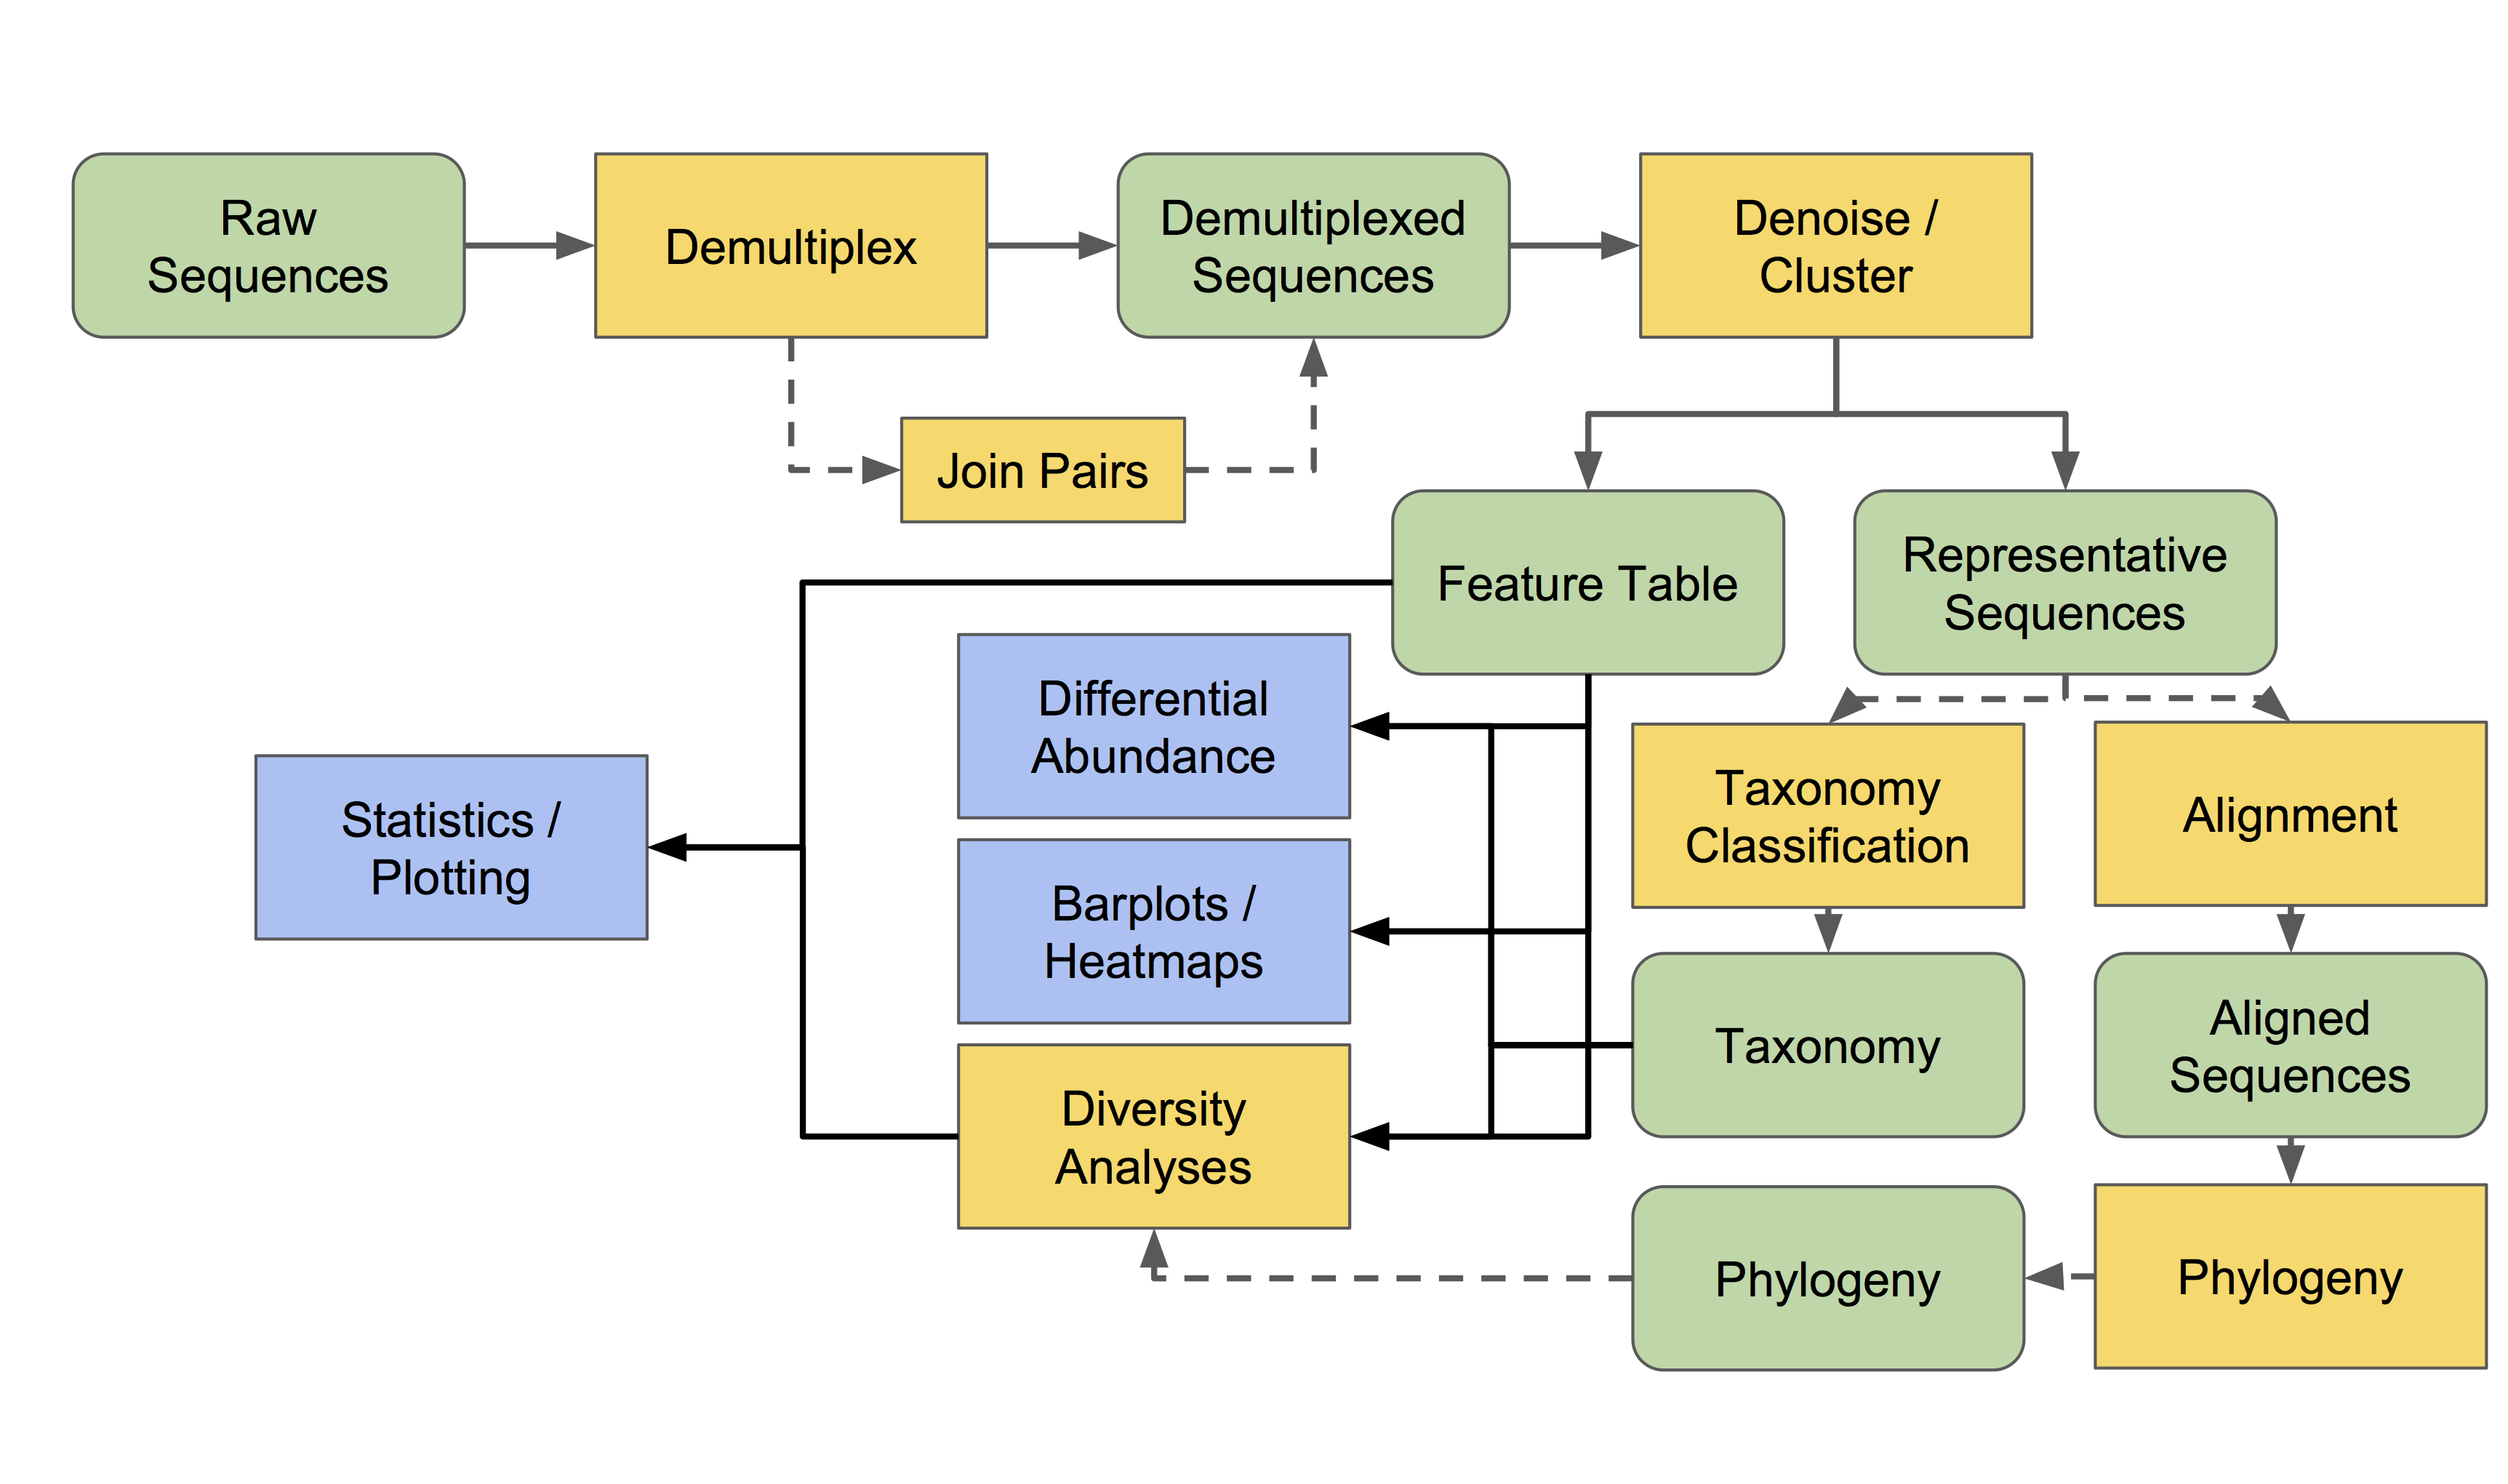
\includegraphics[width=0.8 \linewidth]{figures/qiime.png}
                \caption{A Theoretic Overview of QIIME2 Workflow \protect\cite{qiime1, qiime2}}
                \label{fig:qiime-workflow}
            \end{figure}

            \subsubsection{Denoising techniques}
                There are two denoising techniques provided by QIIME2: DADA2 \cite{DADA1} and Deblur \cite{deblur1}. Major difference between DADA2 and Deblur is a strategy, the strategy used to divide as different species.

                \begin{figure}[p]
                    \centering
                    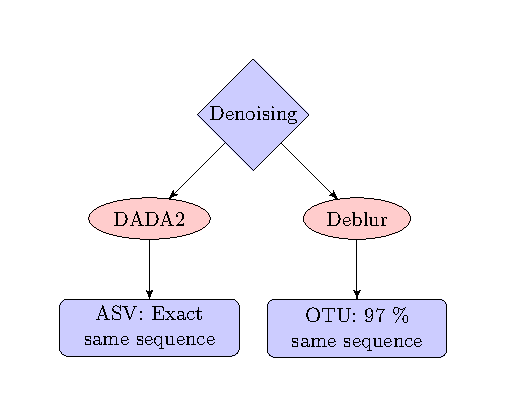
\includegraphics[width=0.5 \linewidth]{figures/denoising/denoising.pdf}
                    \caption{Denoising Techniques which provided by QIIME2}
                    \label{fig:denosing-workflow}
                \end{figure}

            \subsubsection{Taxonomy Classification}

                \begin{figure}[p]
                    \centering
                    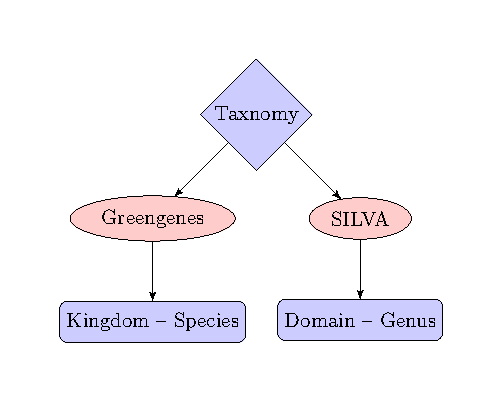
\includegraphics[width=0.5 \linewidth]{figures/taxonomy/taxonomy.pdf}
                    \caption{Taxonomy Classification which provided by QIIME2}
                    \label{fig:taxonomy-workflow}
                \end{figure}

            \subsubsection{Rarefaction}

            \subsubsection{Alpha-diversity}

            \subsubsection{Beta-diversity}

            \subsubsection{ANCOM}
                ANCOM (Analysis of composition of microbiomes) can be used for analyzing the composition of microbiome in multiple populations \cite{ANCOM1}.

                \begin{figure}[p]
                    \centering
                    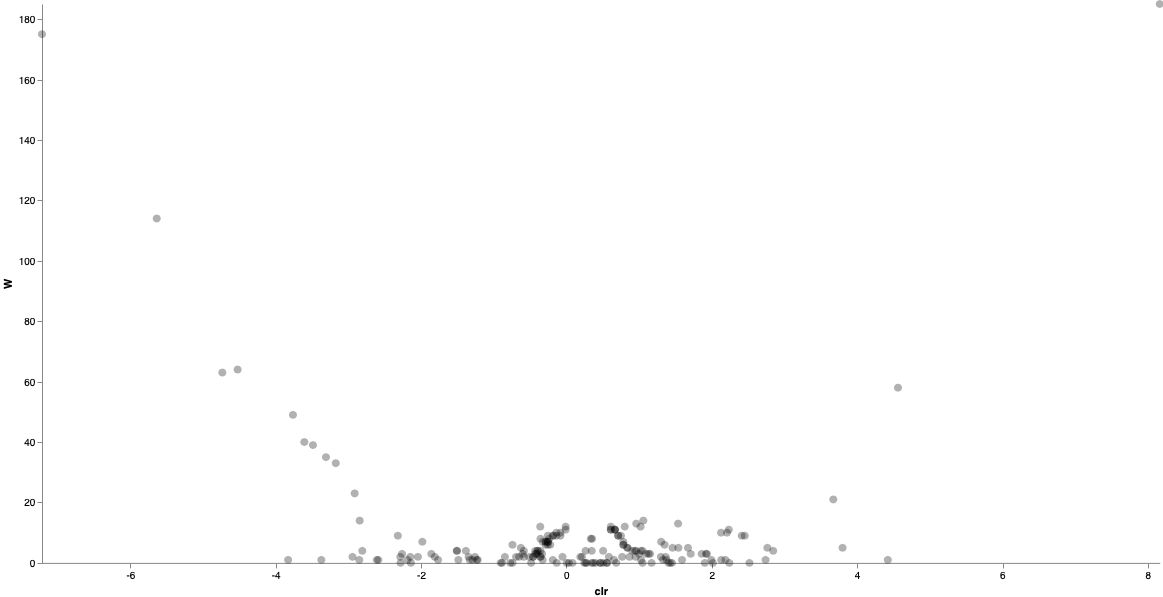
\includegraphics[width=0.8 \linewidth]{figures/ANCOM/example.png}
                    \caption{Example ANCOM Volcano Plot which Provided by QIIME2 \protect\cite{qiime1, qiime2}}
                    \label{fig:ancom-example}
                \end{figure}

        \subsection{Python Packages}

            \subsubsection{Pandas}
                Pandas is a Python package of rich data structures and tools for analyzing with structured data sets \cite{pandas1}.

            \subsubsection{Scikit-learn}
                Scikit-learn grants state-of-the-art implementation of many machine learning algorithms, while controlling an easy-to-use interface tightly integrated the Python code \cite{sklearn1}.

            \subsubsection{Matplotlib}
                Matplotlib is a Python graphics package which used for application development, interactive scripting and publication quality image generation \cite{matplotlib2}. Matplotlib, also, is designed to create simple plots with a few commands \cite{matplotlib1}.

            \subsubsection{Seaborn}
                Seaborn is a Python data visualization package which based on matplotlib, allows a high-level interface for displaying engaging and descriptive statistical graphics \cite{seaborn1}.

    \section{Results}

    \section{Discussion}

    \bibliographystyle{apacite}
    \bibliography{reference}
\end{document}